\section{Planificación del Proyecto}
La planificación del proyecto se llevó a cabo en varias etapas. En primer lugar, se definieron los objetivos generales del sistema y se exploraron las ideas fundamentales que darán forma al proyecto.

Centralmente se tienen tres ramas principales que se pueden observar en la figura \ref{fig:diagrama1}.
\begin{figure}[H]
    \centering
    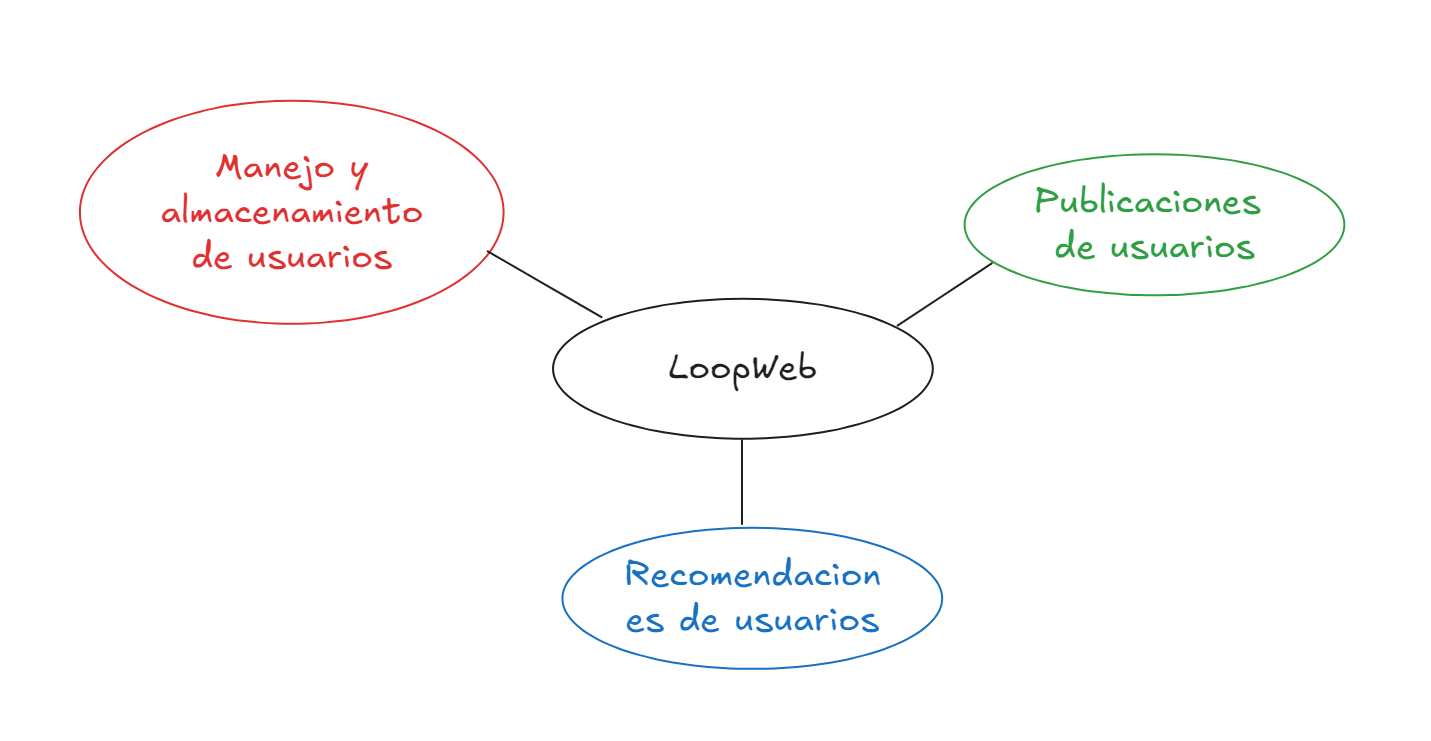
\includegraphics[width=0.5\textwidth]{./src/images/Diagrama1.png}
    \caption{Ejes principales de \loopweb}
    \label{fig:diagrama1}
\end{figure}

A continuación, se presentan los elementos clave que fueron considerados durante esta etapa de planificación:
\begin{enumerate}
    \item \textbf{Creación de perfiles de usuario:} Se busca implementar un sistema básico de perfil de usuario que permite a cada persona en la red social tener una representación digital que contiene:
    \begin{itemize}
        \item Nombre de usuario
        \item Edad del usuario
        \item Nacionalidad del usuario
        \item Géneros musicales que le gustan al usuario
        \item Bandas o artistas que le gustan al usuario (tratadas solo como bandas dentro del programa)
        \item Comentarios que ha realizado el usuario
        \item Amistades del usuario con otros perfiles de la red
    \end{itemize}
    \item \textbf{Establecimiento de conexiones entre usuarios:} Continuando con el punto anterior se busca desarrollar una funcionalidad que permita a los usuarios establecer relaciones de amistad, simulando un comportamiento cercano al de una red social.
    \item \textbf{Publicación y visualización de publicaciones:} Los usuarios podrán crear publicaciones y ver aquellas que estén relacionadas con sus gustos musicales, lo que ``fomentará la interacción'' dentro de la red social.
    \item \textbf{Exploración y recomendación de usuarios:} Este programa permitirá a los usuarios explorar otros perfiles recomendados para ellos (recomendaciones que se basarán en la cercanía de edad y los gustos musicales), lo anterior permitirá promover una experiencia personalizada para cada usuario.
    \item \textbf{Realización de búsquedas eficientes:} Se implementarán algoritmos de búsqueda basados en grafos para permitir la localización eficiente de usuarios dentro de la red social, optimizando la experiencia de navegación.
    \item \textbf{Eficiencia y Escalabilidad:} El sistema será diseñado utilizando estructuras de datos como tablas hash y listas enlazadas, lo que garantiza un rendimiento óptimo incluso con grandes volúmenes de datos.
    \item \textbf{Opción Administrativa:} Se plantea una opción de administración que permitirá gestionar de manera sencilla los usuarios, gustos y sus publicaciones, facilitando el control dentro de la red social así como la creación de nuevos usuarios.
\end{enumerate}

Para una correcta realización del proyecto se crean tres diagramas de flujo que juntos describen el comportamiento esperado de la aplicación.

En la figura \ref{fig:diagrama2} se muestra el diagrama de flujo principal de \loopweb, que se divide en dos partes: un modo de administración (figura \ref{fig:diagrama3}) y otro para la interacción de un usuario en particular (figura \ref{fig:diagrama4}).
\begin{figure}[!h]
    \centering
    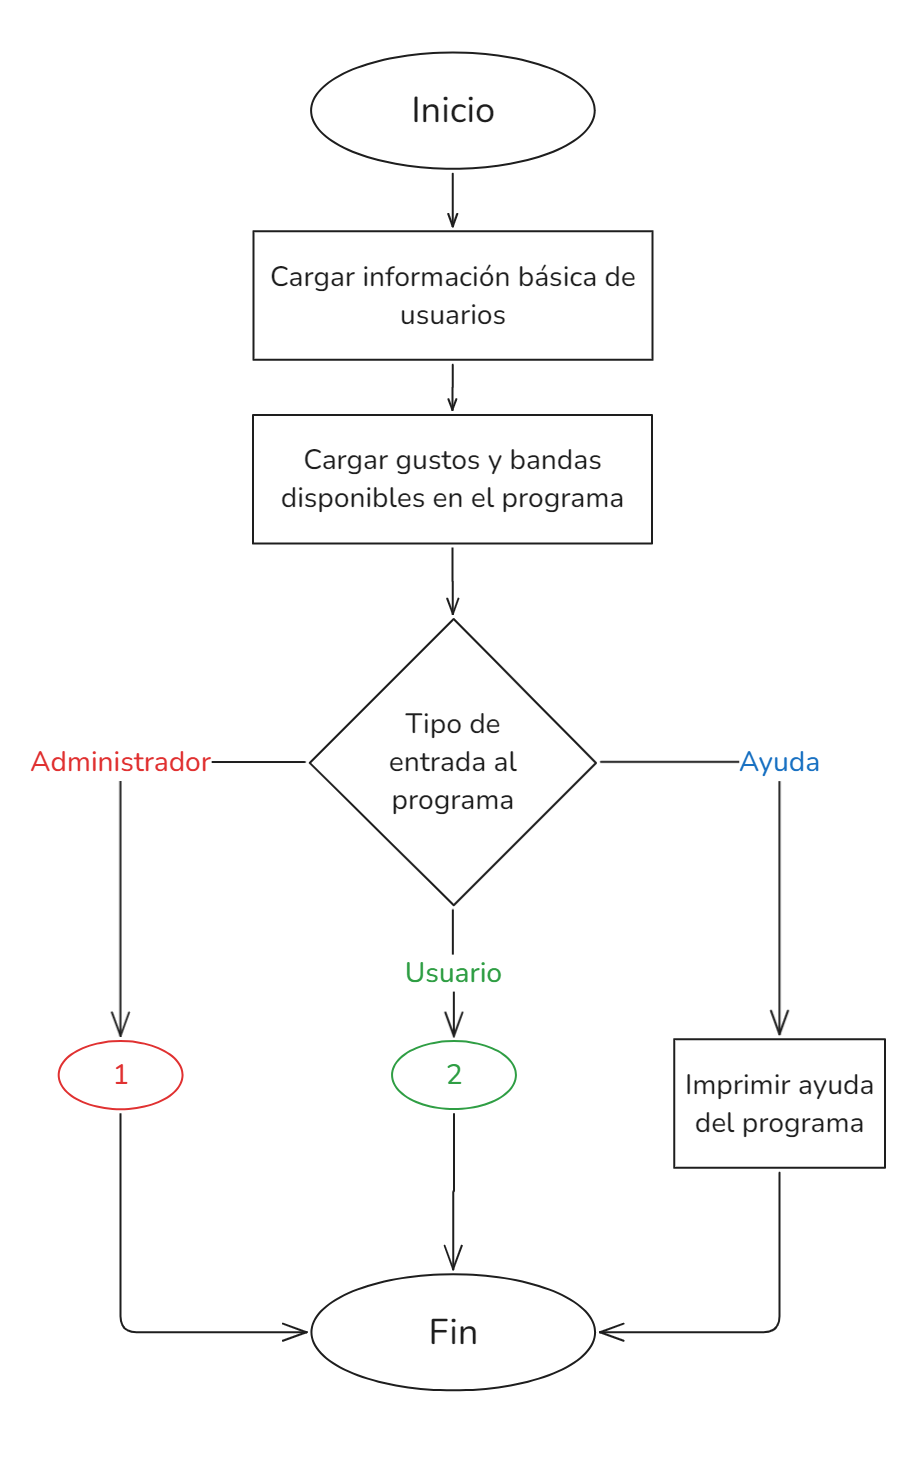
\includegraphics[width=0.3\textwidth]{./src/images/Diagrama2.png}
    \caption{Diagrama de flujo prinicpal de \loopweb}
    \label{fig:diagrama2}
\end{figure}

\begin{figure}[!h]
    \centering
    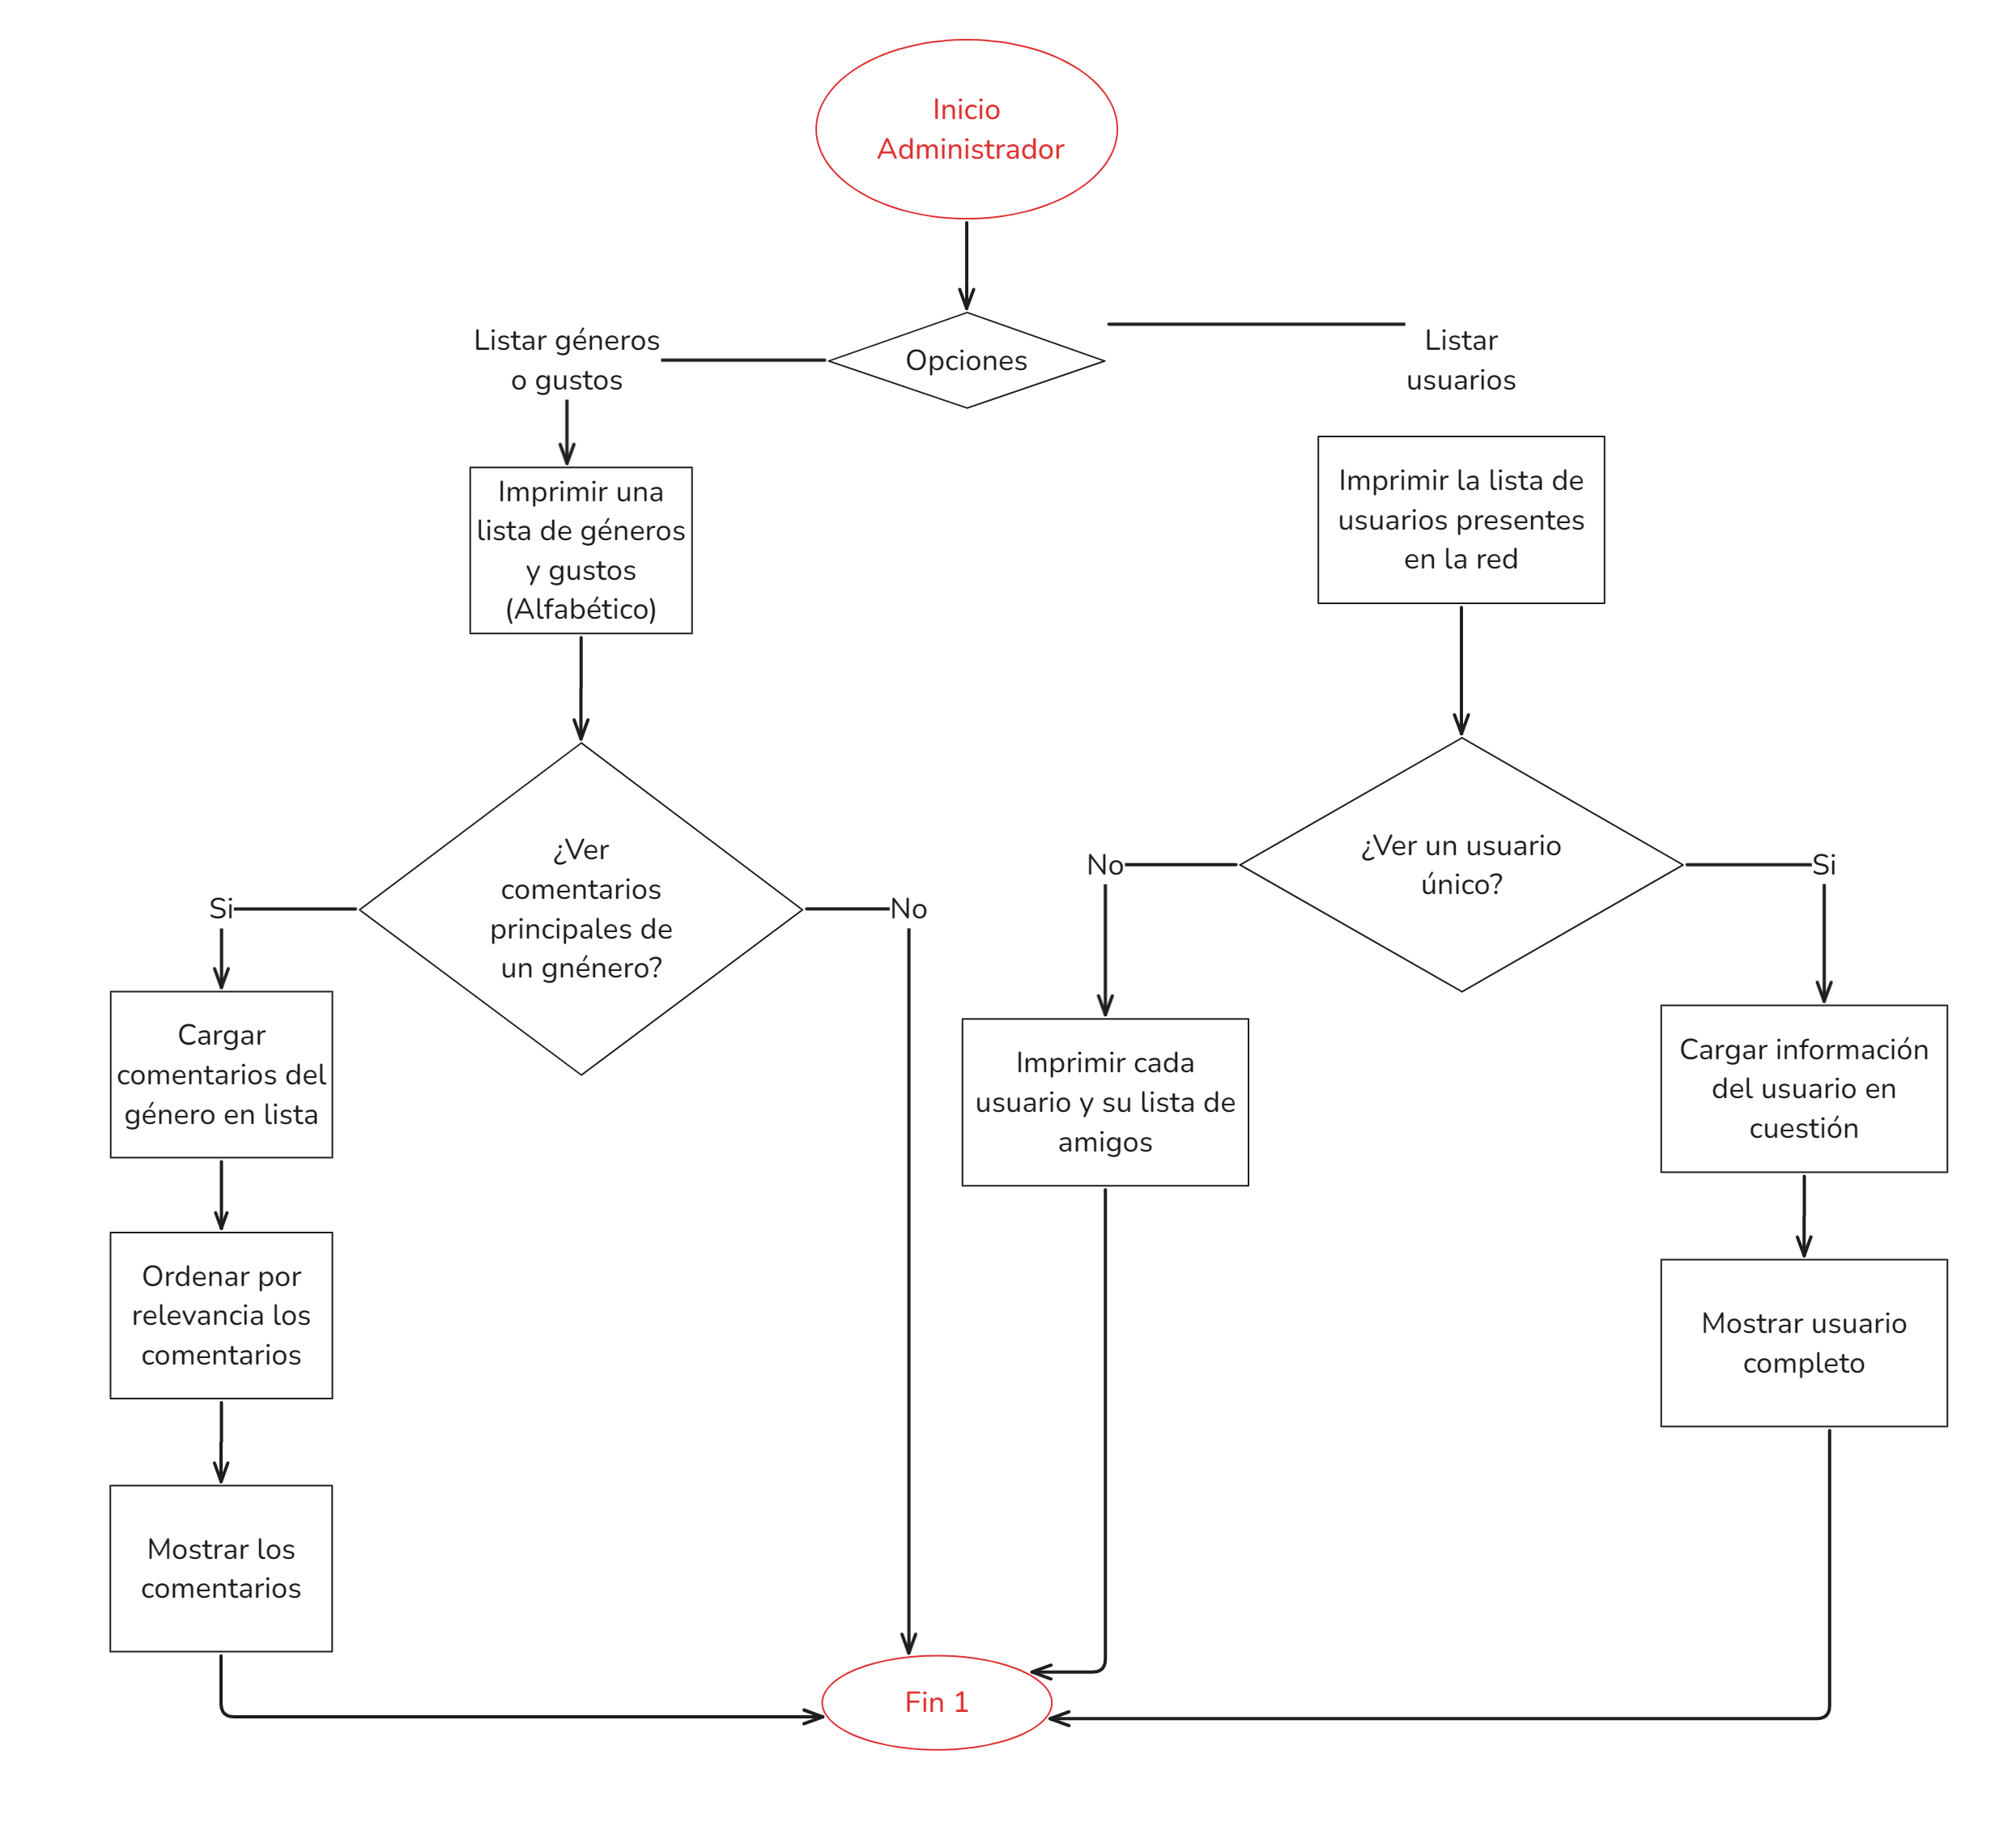
\includegraphics[width=0.5\textwidth]{./src/images/Diagrama3.png}
    \caption{Flujo de un administrador de \loopweb}
    \label{fig:diagrama3}
\end{figure}

\begin{figure}[p]
    \centering
    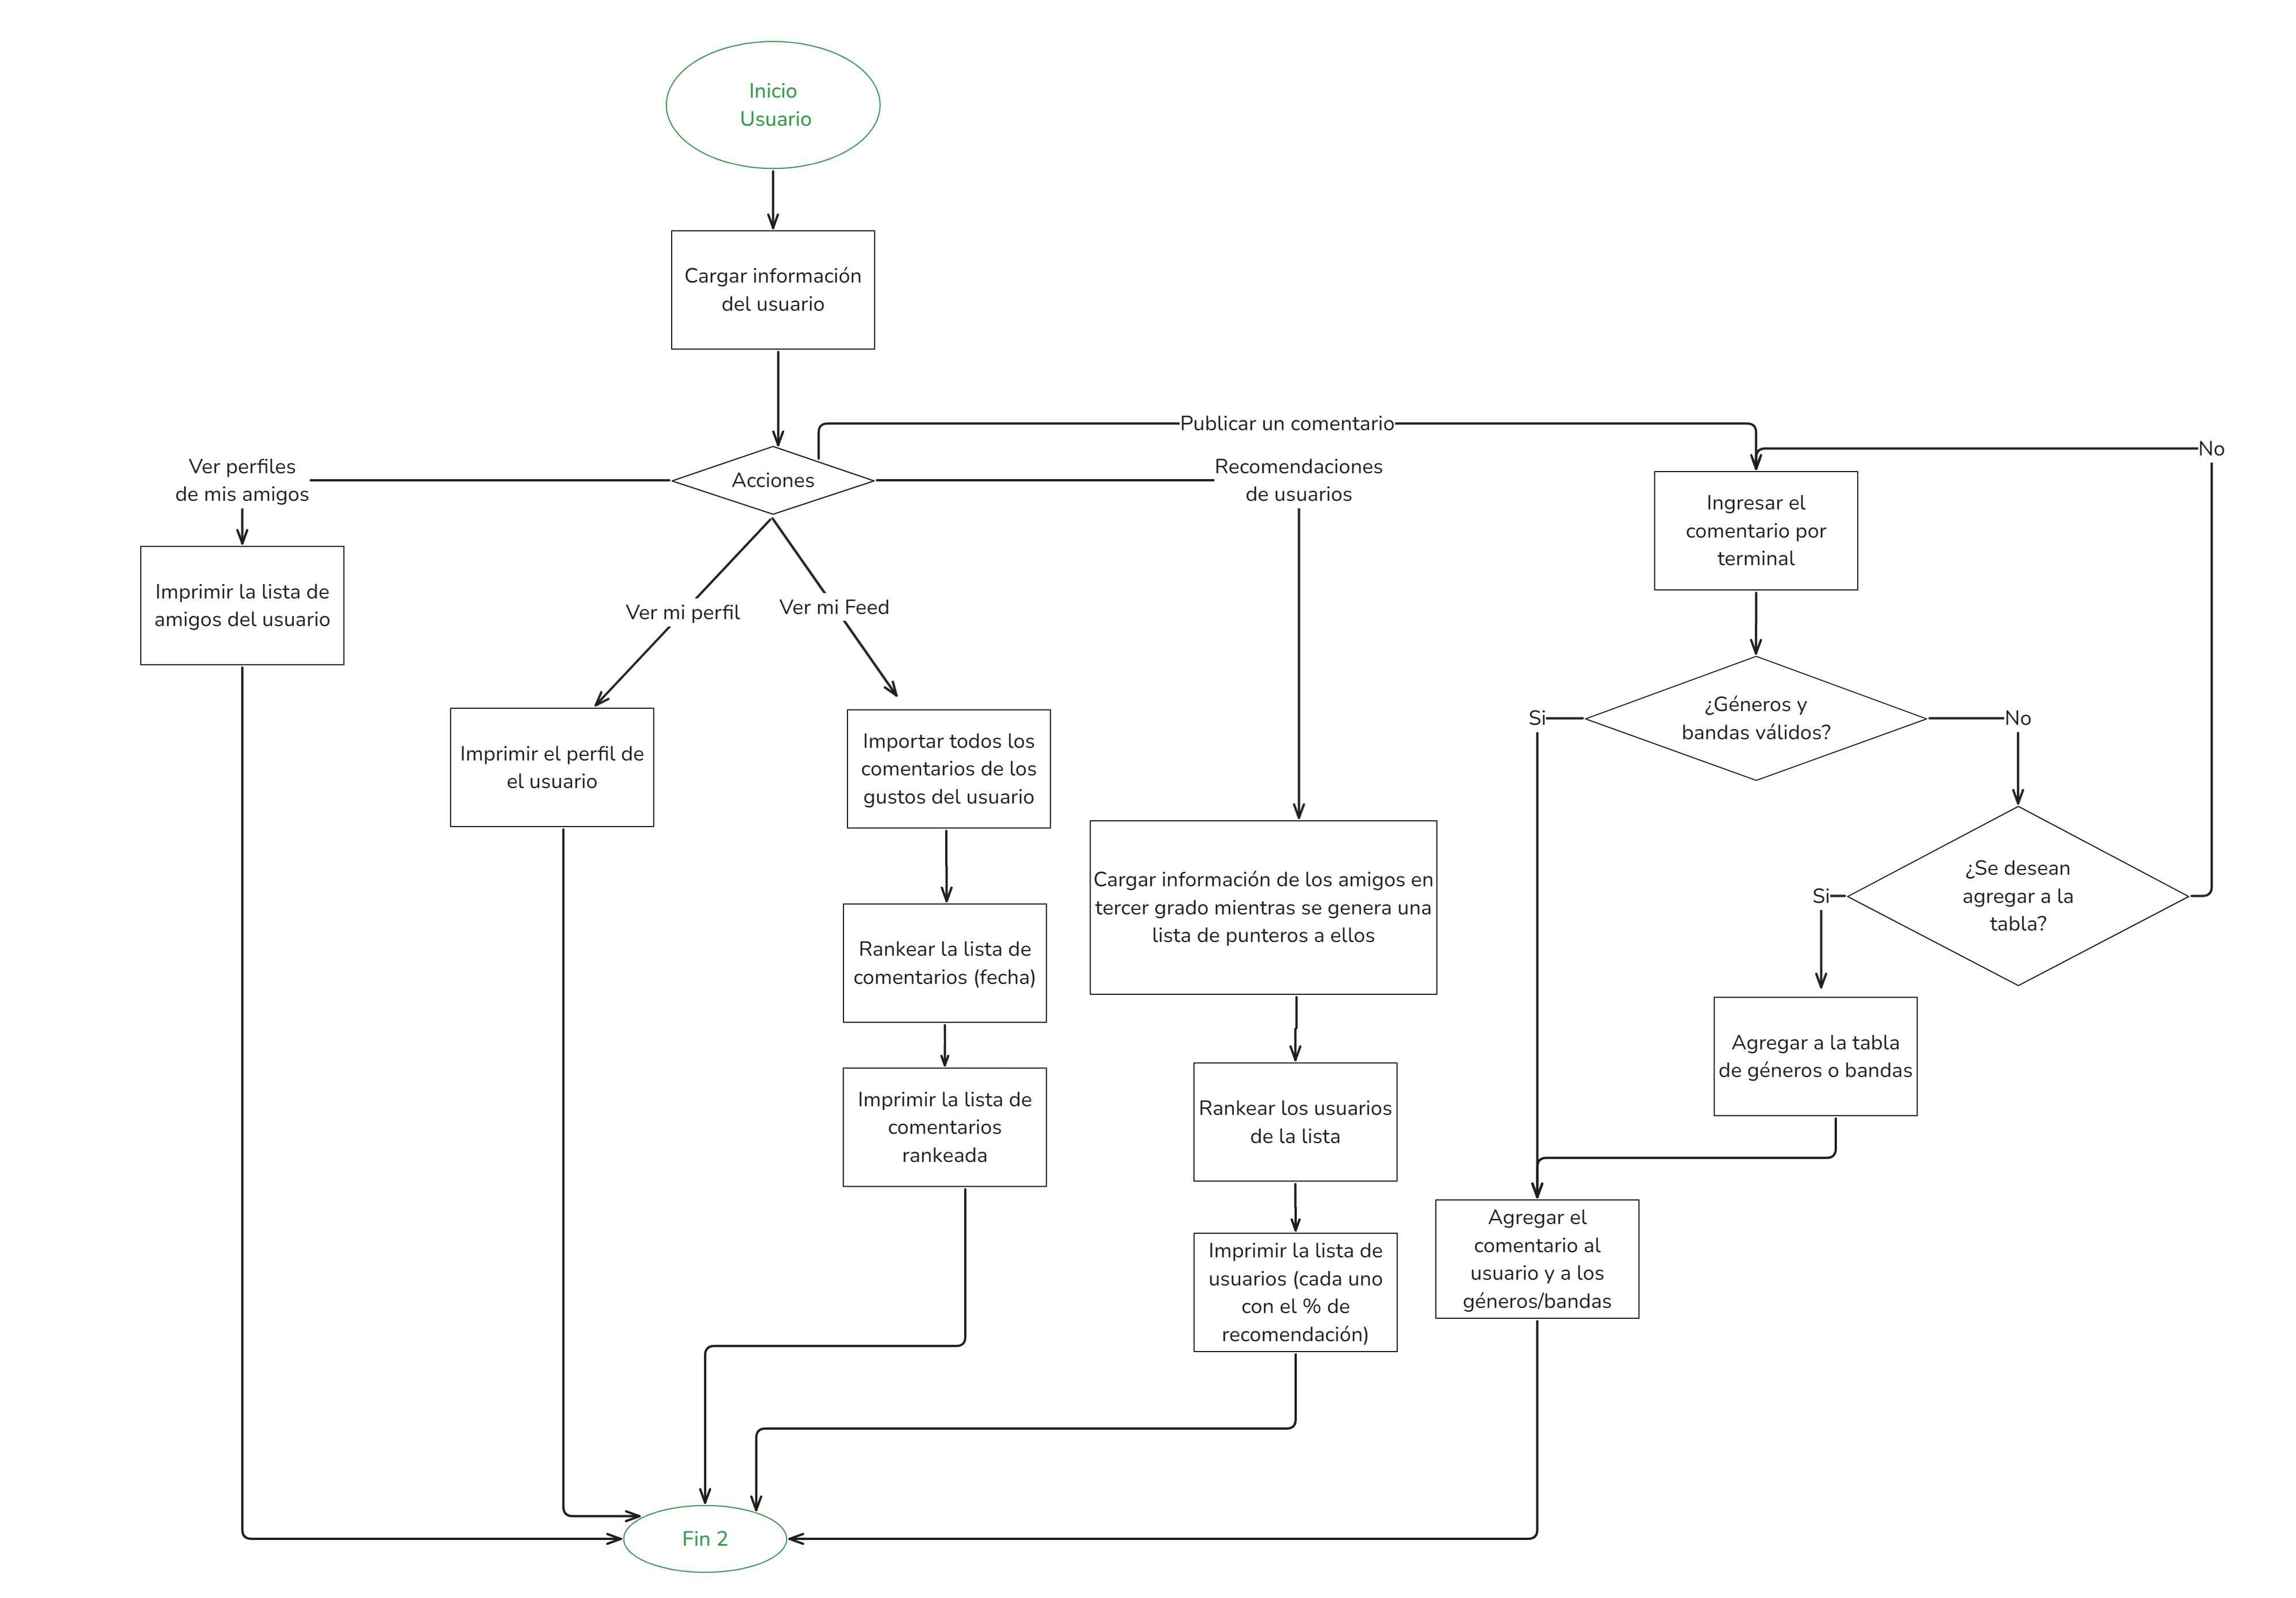
\includegraphics[width=1\textwidth]{./src/images/Diagrama4.png}
    \caption{Flujo de un usuario de \loopweb}
    \label{fig:diagrama4}
\end{figure}

